\newpage
\subsection{Caso d'uso UC2: Autenticazione}
\begin{figure}[h] 
	\centering 
	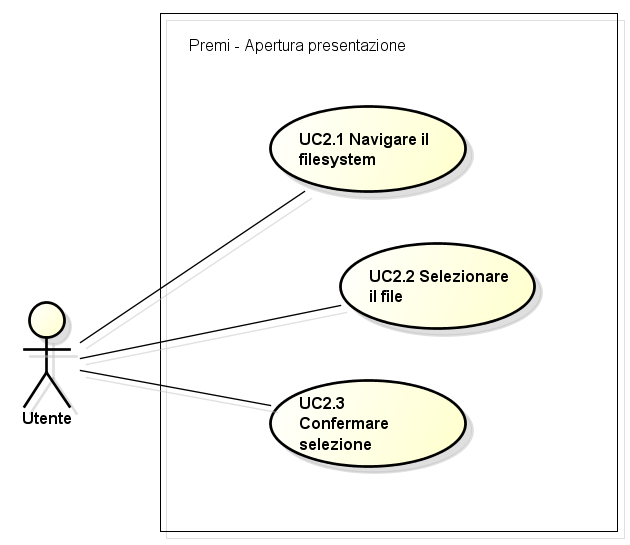
\includegraphics[scale=0.45] {img/UC2.png} 
	\caption{UC2 - Autenticazione} 
\end{figure}

\begin{itemize}
	\item \textbf{Attori:} Utente non autenticato;
	\item \textbf{Scopo e descrizione:} L'utente è già iscritto e vuole avviare la procedura di autenticazione al sito per accedere ai propri file;
	\item \textbf{Precondizione:} L'utente ha selezionato la voce "accedi" presente sul sito;
	\item \textbf{Flusso principale degli eventi:}
	\begin{enumerate}
		\item L'utente inserisce le proprie credenziali [UC2.1];
		\item L'utente conferma l'inserimento dei dati selezionando la voce "login" [UC2.2];
		\item Si può verificare un errore di accesso [UC2.3];
		\item L'utente viene reindirizzato alla propria pagina personale [UC2.4].
	\end{enumerate}
	\item \textbf{Postcondizione:} Il sistema verifica le credenziali inserite e permette all'utente di accedere alla sua pagina personale.
\end{itemize}

\newpage

\subsection{Caso d'uso UC2.1: Inserimento credenziali}
\begin{figure}[h] 
	\centering 
	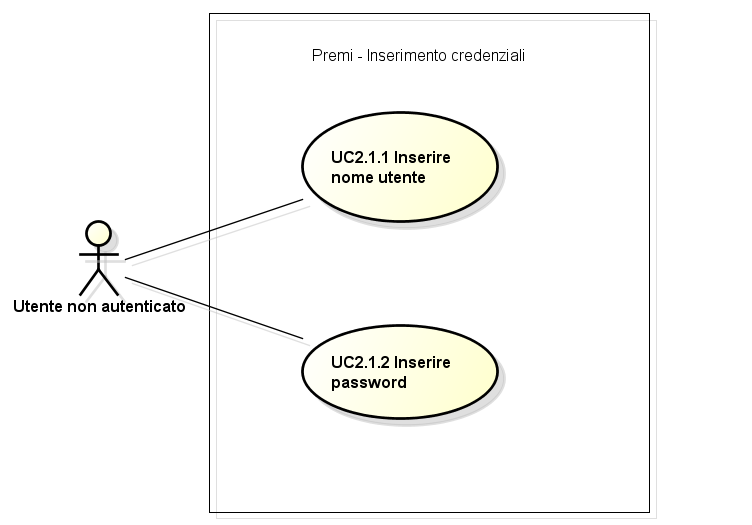
\includegraphics[scale=0.45] {img/UC2.1.png} 
	\caption{UC2.1 - Inserimento credenziali} 
\end{figure}
\begin{itemize}
	\item \textbf{Attori:} Utente non autenticato;
	\item \textbf{Scopo e descrizione:} L'utente inserisce nome utente e password per poter accedere al sito;
	\item \textbf{Precondizione:} L'utente visualizza la schermata di inserimento dei dati richiesti per l'accesso;
	\item \textbf{Flusso principale degli eventi:}
	\begin{enumerate}
		\item L'utente inserisce il proprio nome utente [UC2.1.1];
		\item L'utente inserisce la propria password [UC2.1.2];
	\end{enumerate}
	\item \textbf{Postcondizione:} Tutti i campi richiesti sono stati compilati correttamente.
\end{itemize}

\subsection{Caso d'uso UC2.1.1: Inserire nome utente}
\begin{itemize}
	\item \textbf{Attori:} Utente non autenticato;
	\item \textbf{Scopo e descrizione:} L'utente inserisce il proprio nome utente;
	\item \textbf{Precondizione:} La casella dove inserire il nome utente è vuota;
	\item \textbf{Postcondizione:} La casella è stata compilata con il nome utente inserito dall'utente.
\end{itemize}

\subsection{Caso d'uso UC2.1.2: Inserire password}
\begin{itemize}
	\item \textbf{Attori:} Utente non autenticato;
	\item \textbf{Scopo e descrizione:} L'utente inserisce la propria password;
	\item \textbf{Precondizione:} La casella dove inserire la password è vuota;
	\item \textbf{Postcondizione:} La casella è stata compilata con la password inserita dall'utente.
\end{itemize}

\subsection{Caso d'uso UC2.2: Accesso}
\begin{itemize}
	\item \textbf{Attori:} Utente non autenticato;
	\item \textbf{Scopo e descrizione:} L'utente conferma le credenziali inserite scegliendo di effettuare l'accesso tramite il tasto di login;
	\item \textbf{Precondizione:} Nome utente e password sono stati inseriti;
	\item \textbf{Postcondizione:} Il sistema verifica i dati inseriti.
\end{itemize}

\subsection{Caso d'uso UC2.3: Errore di autenticazione}
\begin{itemize}
	\item \textbf{Attori:} Sistema;
	\item \textbf{Scopo e descrizione:} L'utente ha inserito delle credenziali errate e il sistema blocca l'accesso, riportando l'utente alla schermata di accesso;
	\item \textbf{Precondizione:} Nome utente e password sono stati inseriti in modo errato;
	\item \textbf{Postcondizione:} Il sistema riporta l'utente alla schermata di accesso.
\end{itemize}

\subsection{Caso d'uso UC2.4: Dati inseriti correttamente}
\begin{itemize}
	\item \textbf{Attori:} Sistema;
	\item \textbf{Scopo e descrizione:} Il sistema ha verificato che le credenziali inserite sono corrette;
	\item \textbf{Precondizione:} Nome utente e password sono stati inseriti;
	\item \textbf{Postcondizione:} Il sistema ha verificato che i dati inseriti sono corretti.
\end{itemize}

\subsection{Caso d'uso UC2.5: Reindirizzamento a pagina personale}
\begin{itemize}
	\item \textbf{Attori:} Sistema;
	\item \textbf{Scopo e descrizione:} Il sistema dopo aver consentito l'accesso all'utente mostra la sua pagina personale;
	\item \textbf{Precondizione:} Nome utente e password sono stati inseriti correttamente;
	\item \textbf{Postcondizione:} Il sistema mostra la pagina personale dell'utente.
\end{itemize}

\newpage